This section implements the Todo application using the MobX package in order to handle the state.

\subsubsection{Base funtionalities}  \label{par:todo_app_inherited_widget_introduction} 
 
As mentioned in Chapter XX RIFERIMENTO the MobX package makes one or more parts of the state Observable and uses a particular widget, called Observer, to keep track of changes in the observed variables. To be able to define observables is necessary to extend the intrested class with the Store class offedered by the MobX package. Moreover, the container class must be made abstract. The usual definition of the Todo class is used momentarily remembering that no rendering optimizations are kept into account. The parts of the state to be made observable are: the list of todos,  the filter and the tab value. The whole application, indeed, relies on them to track changes and update correspondingly. 
\paragraph{The observable state - }
\label{subpar:todo_app_bloc_core_state}A new abstract class is created and called \_TodoStore. It contains the list of todos and the filter. A separate observable variable will be used to implement the state of the tab. This design choice allows to present two different approaches the MobX package provides and divides the information regarding the todos from the information regarding the tab value. ( the filter value is in some way connected with the list of todo). This new abstract class is extended with the Store class. A list of todos and a visibility filter are created inside it and annoted with the @observable syntax. The @observable annotation informs the code generator that those variables need to be made observable, moreover, the code generator automatically creates a getter and a setter action for them. 
\begin{code}
\mbox{}\\
\captionof{listing}{Todo app - MobX- TodoStore abstract class implementation} \mbox{}
		\label{code:2.14}
\begin{minted}[bgcolor=bluepoli!10]{dart}
//extend with the Store mixin to allow annotations
abstract class _TodoStore with Store {
  @observable
  List<Todo> todos = [];

  @observable
  VisibilityFilter filter = VisibilityFilter.all;
}
\end{minted}
\mbox{}
\end{code}

\paragraph{Actions - }
\label{subpar:todo_app_bloc_core_state}In this implementation the strict mode is set to “always”. This choice reflects the common usage of the pattern. It is indeed a common choice to allow state mutations only through actions. This behavior comes with a lot of advantages that make it the correct choice for the major of the cases. This subject will be deeper investigated in the latter sections but, for the moment,  it is worth noting that the MobX package also provides the possibility to configure the strict mode to “never”  allowing the direct change of the state without passing through an action.  A bunch of new methods are now added to the TodoStore class and marked with the @action annotation. The simplest one is the \textit{changeFilter} method that allows to change the current filter.
\begin{code}
\mbox{}\\
\captionof{listing}{Todo app - MobX - TodoStore's \textit{changeFilter} action implementation} \mbox{}
		\label{code:2.14}
\begin{minted}[bgcolor=bluepoli!10]{dart} 
 @action
  void changeFilter(VisibilityFilter filter) {
    this.filter = filter;
  }
\end{minted}
\mbox{}
\end{code}

A method to set the \textit{completed} field of a particular todo is also required. This method is called \textit{setCompleted} and takes the id of the todo to be changed and its new completed value. As usual,  a new list is created, after modifying the todo, in order to allow MobX to recognize the change in the list of todos.
\begin{code}
\mbox{}\\
\captionof{listing}{Todo app - MobX - TodoStore's \textit{setCompleted} action implementation} \mbox{}
		\label{code:2.14}
\begin{minted}[bgcolor=bluepoli!10]{dart}
@action
  void setCompleted(int id, bool completed) {
    //check the todo's existance
    assert(todoExists(todos,id) ==true, 'No todo with id : \$id');
    todos.where((element) => element.id==id).first.completed=completed;
  }

\end{minted}
\mbox{}
\end{code}

The two usual methods to fetch and save todos into the DataBase/repository are implemented and annotated with the @action annotation too.
\begin{code}
\mbox{}\\
\captionof{listing}{Todo app - MobX - TodoStore's \textit{fetchTodos} and \textit{saveTodos} actions implementation} \mbox{}
		\label{code:2.14}
\begin{minted}[bgcolor=bluepoli!10]{dart}
@action
Future<void> fetchTodos() async {
  todos = await TodoRepository.loadTodos();
}

@action
Future<void> saveTodos() async {
  await TodoRepository.saveTodos(todos);
}
\end{minted}
\mbox{}
\end{code}

\paragraph{Computed fields - }
\label{subpar:todo_app_bloc_core_state}computed fields are the part of the state that can be derived from other parts of the state. They are pivotal in the MobX state management solution because the package is able to smartly compute them and to perform lot of optimizations under the hood using memoization technique to prevent useless computations. They are a similar concept with respect to selector in Redux. The list of completed todos is well suited to demonstrate the power of the computed field. A new getter function is created and called \textit{completedTodos}. It computes the list of completed todos and returns it. The @computed annotation is positioned right above the method to let the code generator know how to implement it in order to perform the optimizations discussed earlier. During the application lifecycle the \textit{completedTodos} method will be accessed numerous times and automatically recomputed in case a part of the state, it depends on, changes. Moreover, its value is memoized and reused in case multiple accesses are necessary. Another method is created in the same way in ordert to compute the \textit{pendingTodos}.
\begin{code}
\mbox{}\\
\captionof{listing}{Todo app - MobX - TodoStore's \textit{completedTodos} and \textit{pendingTodos }computed values implementation} \mbox{}
		\label{code:2.14}
\begin{minted}[bgcolor=bluepoli!10]{dart}
@computed
List<Todo> get completedTodos =>
    todos.where((element) => element.completed).toList();

@computed
List<Todo> get pendingTodos =>
    todos.where((element) => !element.completed).toList();
\end{minted}
\mbox{}
\end{code}


\textit{pendingTodos} and \textit{completedTodos} methods are then used to implement other computed values: the \textit{filteredTodos}, the number of completed todos and the number of pending todos. The \textit{filteredTodos} method returns the list of todos that match the visibility filter. It is composed using the computed values defined before. Also the \textit{stats} value can be obtained using the computed feature.
\begin{code}
\mbox{}\\
\captionof{listing}{Todo app - MobX - \textit{filteredTodos} and \textit{stats} computed value implementation} \mbox{}
		\label{code:2.14}
\begin{minted}[bgcolor=bluepoli!10]{dart}
@computed //compute todos list length
int get len => todos.length;

@computed //compute the completed todos
int get completed => completedTodos.length;

@computed //compute the pending todos
int get pending => pendingTodos.length;

@computed //compute the filtered list
List<Todo> get filteredTodos {
  switch (filter) {
    case VisibilityFilter.all:
      return todos;
    case VisibilityFilter.completed:
      return completedTodos;
    case VisibilityFilter.notCompleted:
      return pendingTodos;
  }
}

@computed //compute stats
String get stats {
  return completed.toString();
}
\end{minted}
\mbox{}
\end{code}

\paragraph{The code generation - }
\label{subpar:todo_app_bloc_core_state}The \_TodoStore class won’t be directly used in the code but its actual implementation will. The \_TodoStore is, indeed, an abstract class and is used by the code generator to implement the TodoStore class. A particular line of code must be placed just below the imports to allow the code generator to recognize the abstract class to be implement. This line of code uses the \textit{part} directive followed by the name of the file to be generated. The generated code will be putted inside a file called \textit{counter.g.dart }which is included with the \textit{part} directive right below the imports. Without this line, the code generator will not produce any output. The generated file contains the \_\$TodoStore mixin. It is combined with the \_TodoStore abstract class to finally implement the TodoStore class.
\begin{code}
\mbox{}\\
\captionof{listing}{Todo app - MobX - TodoStore code generation} \mbox{}
		\label{code:2.14}
\begin{minted}[bgcolor=bluepoli!10]{dart}
//allow the code generator to create the todo_store.g.dart file
part 'todo_store.g.dart';
//use the generater file
class TodoStore = _TodoStore with _\$TodoStore;
\end{minted}
\mbox{}
\end{code}

In order to use the code generator and generate the code, a series of directives can be inserted into the terminal. For the sake of simplicity, the following line of code will be always used to generate code.
\begin{code}
\mbox{}\\
\captionof{listing}{Todo app - MobX - directive for code generation} \mbox{}
		\label{code:2.127}
\begin{minted}[bgcolor=bluepoli!10]{dart}
flutter pub run build_runner watch --delete-conflicting-outputs
\end{minted}
\mbox{}
\end{code}

It automatically generates the code and handles all the possible conflicts that can arise. For example, in case a file named todo\_store.g.dart already exists it first deletes the file and then computes it again. With this line of code, the code generation process is made really easy. The drawback is that every time the code is modified the generated code is re-created from scratch. In our case this does not represent a big deal because the application is contained and the code generator only takes about 12-13 seconds to execute and create the entire code. In a more spread scenario other directives can be used to make the code generation process lighter. I decided not to show the generated code because it is quite long and hard to read.

\paragraph{The spy feature - }
\label{subpar:todo_app_bloc_core_state} in order to enable the spy feature a new configuration for the \textit{mainContext} must be provided before running the application, in the main function. After cloning the default \textit{mainContext} the \textit{isSpyEnabled} field is set to true and the \textit{writePolicy} field  is set to always in order to enable the strict-mode for every state change. Moreover, a function must be passed to the spy feature. The code inside this function is executed every time an action occurs. In our case is enough to print the event name when an event of type \textit{action} occurs to have a clear picture of what is going on.

\begin{code}
\mbox{}
\captionof{listing}{Todo app - MobX - spy feature attachment} \mbox{}
		\label{code:2.14}
\begin{minted}[bgcolor=bluepoli!10]{dart}
//create a new configuration with strict mode set to "always"
mainContext.config = mainContext.config
    .clone(isSpyEnabled: true, writePolicy: ReactiveWritePolicy.always);
//provide a function to the spy feature
mainContext.spy((event) {
  if (event.type == "action") {
    print("event name : " + event.name);
  }
});
\end{minted}
\mbox{}
\end{code}


And that’s basically all we need in order to implement the application’s state. At this point is already possible to test the state logic.

\paragraph{Making the state accessible - }
\label{subpar:todo_app_bloc_core_state} MobX, like every other solution used so far, uses a Provider widget to supply the state to the subtree. In this case the mobx package do not self-implement the provider widget, instead it relies on and external package called \textit{Provider} which offers this feature. The procedure is the usual one, the MaterialApp widget is wrapped into a Provider widget of type TodoStore which supplies the instance of the TodoStore to the subtree. It has a \textit{create} field where the TodoStore can be initialized and where the fetching of todos can take place.
\begin{code}
\mbox{}\\
\captionof{listing}{Todo app - MobX - making the state accessible using the Provider widget} \mbox{}
		\label{code:2.14}
\begin{minted}[bgcolor=bluepoli!10]{dart}
//wrap the material app into a Provider widget
return Provider<TodoStore>(
    create: (_) => TodoStore()..fetchTodos(), //fetch todos at creation
    child: MaterialApp(. . .),
    }));
\end{minted}
\mbox{}
\end{code}



\paragraph{The HomePage and the TabSelector component - }
\label{subpar:todo_app_bloc_core_state}The HomePage is almost entirely built using the state's part regarding the tab. The first thing to do is to create an observable variable of type TabState to represent it. This time, a different approach with respect to the one used to implement the state of the todos and the filter, is used. We are not creating an abstract class neither generating any code. Moreover, no Provider widget is used because the tab value needs to be accessed only in a couple of widgets and passing it between them is way easier. The tab value is wrapped into an observable object of type TabState. The entire object is managed by the MobX package and the only difference with respect to a normal variables usage is that, in order to access the TabState value, we need to further dig into the \textit{value} field instead of just using the tab variable as it is. Both the body and the VisibilityFilterSelector widget  as well as the TabSelector widget depends on the tab value so the entire Scaffold widget is wrapped into a Observer widget. Once a change in the \textit{tab} variable occurs, the Observer widget automatically determine which parts of the Scaffold widget should be rebuilt. In our case all components depends on the tab value and then are rebuilt once a tab change occurs. In cases independent components are wrapped into the Observer widget they would not be rebuilt. The entire Scaffold widget is populated using the tab variable as usual. The only part that differs is the TabSelector component. Beside depending on the tab value it also needs to change it. There are two equivalent options : passing the tab variable to the TabSelector component or passing a closure function. The first solution is used. 
\begin{code}
\mbox{}\\
\captionof{listing}{Todo app - MobX - HomePage implementation} \mbox{}
		\label{code:2.14}
\begin{minted}[bgcolor=bluepoli!10]{dart}
class HomePage extends StatelessWidget {
  HomePage({Key? key}) : super(key: key); 
  //new observable variable
  final _tab = Observable<TabState>(TabState.todos);

 @override
  Widget build(BuildContext context) {
    print("building HomePage");
    return Observer(//wrap the HomePage into a Observer widget
      builder: (context) {
        return Scaffold(
          appBar: AppBar(
            title: const Text("Todo App"),
            actions: [
             _tab.value == TabState.todos //access the state here
                    ? const VisibilityFilterSelector()
                    : Container()

            ],
          ),
          //access the state here
          body: _tab.value == TabState.todos ? const TodoView() :
           const Stats(),
          bottomNavigationBar: TabSelector(),
          floatingActionButton:  _tab.value == //access the state here
           TabState.todos
                ? FloatingActionButton(...)
                : Container()

        );
      }
    );
  }
}
\end{minted}
\mbox{}
\end{code}

A new variable is added to the TabSelector widget and populated in the constructor. It is used in the \textit{onTap} field’s function to mutate the tab value once the user taps on one specific BottomNavigationBarItem widget. Notice that the state change is wrapped into a \textit{runInAction} object. This because if we change the tab value directly, a run time error would arise alerting that observable values cannot be changed outside actions. This is due to the strict mode previously set to "always". \textit{runInAction} creates a throwaway action we can use directly in the code. This approach is made necessary because we used a stand alone Observable variable. If we included the tab variable into the TodoStore class the code generator would had automatically create its getter and setter actions.


\begin{code}
\mbox{}\\
\captionof{listing}{Todo app - MobX - TabSelector component implementation} \mbox{}
		\label{code:2.14}
\begin{minted}[bgcolor=bluepoli!10]{dart}

class TabSelector extends StatelessWidget {
  //new variable passes from the HomePage
  final Observable<TabState> tab; 

  const TabSelector({Key? key, required this.tab}) : super(key: key);

  @override
  Widget build(BuildContext context) {
    print("building TabSelector");

      return BottomNavigationBar( 
        //use it here
        currentIndex: TabState.values.indexOf(tab.value),
        onTap: (index) {
          //use a runInAction necessary for the strict mode
          runInAction(() => tab.value = TabState.values.elementAt(index));
        },
        items: (...),
      );
  }
}
\end{minted}
\mbox{}
\end{code}
\paragraph{The VisibilityFilterSelector component - }
\label{subpar:todo_app_bloc_core_state}It entirely depends on the value of the filter in the TodoStore. To obtain the instance of the TodoStore we use the static \textit{of} method of the Provider widget specifying the type of the instance we are looking for. This procedure will be frequently used from now on and is usually performed at the beginning of the \textit{build} method. 
\begin{code}
\mbox{}\\
\captionof{listing}{Todo app - MobX - retrieving the TodoStore} \mbox{}
		\label{code:2.132}
\begin{minted}[bgcolor=bluepoli!10]{dart}
final store = Provider.of<TodoStore>(context);
\end{minted}
\mbox{}
\end{code}

The entire VisibilityFilterSelector component is then populated using the filter  variable contained in the TodoStore as usual and wrapped into an Observer widget to make is responsive to filter changes. In the \textit{onChanged} field of the DropdownMenuItem widgets the \textit{changeFilter} action previously defined is used to
set the filter value to the tapped one.
\begin{code}
\mbox{}\\
\captionof{listing}{Todo app - MobX - VisibilityFilterSelector component implementation} \mbox{}
		\label{code:2.133}
\begin{minted}[bgcolor=bluepoli!10]{dart}
return Observer( //wrap the VisibilityFilterSelector into a Observer widget
  builder: (context) {
    print("building Visibilityfilter");

    return DropdownButton<VisibilityFilter>(
      value: store.filter, //use the state here
      items: (...),
      onChanged: (tappedValue) {
        //change the state here
        store.changeFilter(tappedValue!);
      },
    );
  },
);
\end{minted}
\mbox{}
\end{code}

Notice that we could omit the usage of the \textit{changeFilter} action and set the value of the filter directly. This because a setter and a getter action are automatically created by the code generator for every observable field. This implies that the \textit{changeFilter} action could also be omitted in the definition of the TodoStore abstract class.
\begin{code}
\mbox{}\\
\captionof{listing}{Todo app - MobX - changing the state in the VisibilityFilterSelector without predefined action} \mbox{}
		\label{code:2.134}
\begin{minted}[bgcolor=bluepoli!10]{dart}
onChanged: (tappedValue) {
        //another way of changing the state
        store.filter = tappedValue!; 
      },
\end{minted}
\mbox{}
\end{code}

I personally dislike this feature MobX package offers in the Flutter framework. I investigated a bit in the usage of MobX with React and JS finding out that, in that case, it behaves as expected raising a warning in case a field is directly changed. (violating the strict mode) I find the way for changing the filter value proposed in the Source Code \ref{code:2.133} a lot more elegant with respect to the one proposed in the Source Code \ref{code:2.134}. Explicitly using predefined actions, indeed, brings way more meaning for the reader and prevents programmers to accidentally mutate the state in the implementation process. Even if I prefer the first approach, in the end,  both approaches pass though actions in order to change the state and this respects the MobX's rules. Actions are, indeed, really important to the correct functioning of the application because using them allows the MobX package to generate atomic state transitions. Suppose a simple action, like the one we just used,  produces reactions of different types and those reactions affects different parts of the state and the UI. Suppose now that the strict mode is disabled and set to "never". In that case, the various reactions can be completed/fired in different interval of time because their carried computation is heavier of lighter with respect of the others. Consequently the entire state of the application is not well synchronized and the UI could reflect this inconsistency bringing to a bad situations. MobX package ensure that actions, and consequent reactions, are performed atomically without leaking any intermediate values as long as actions are used.
\paragraph{The Stats component - }
\label{subpar:todo_app_bloc_core_state} this component is really simple. It just needs to access the TodoStore to get the \textit{stats} value. The procedure shown in the Source Code \ref{code:2.132} is used as usual to get an instance of the TodoStore and, consequently, of the \textit{stats} value. The entire widget is then wrapped into an Observer widget .
\begin{code}
\mbox{}\\
\captionof{listing}{Todo app - MobX - Stats component implementation} \mbox{}
		\label{code:2.14}
\begin{minted}[bgcolor=bluepoli!10]{dart}
//retrive the state
final store = Provider.of<TodoStore>(context);
return Observer(//wrap the Stats component into an Observer widget
  builder: (context) {
           //access the state
           return Center(child: Text(store.stats));
  },
);
\end{minted}
\mbox{}
\end{code}
\paragraph{The TodoView component and the TodoItem component - }
\label{subpar:todo_app_bloc_core_state} These two components represent the core of the UI development process. Remember now that no optimizations are considered for the moment. The TodoView widget needs to access the state and to re-render once a change in the \textit{filteredtodos} list occurs. In this scenario, the MobX pattern really shines. It is sufficient to wrap the entire TodoView widget inside a Observer widget and access the filtered list contained in the TodoStore to allow the MobX package to automatically detect a change in the filtered list. Once the list of todos or the filter is updated, the \textit{filteredTodos} list is automatically re-computed. As usual the TodoItem widget just acts as a visualizer for the corresponding todo and consequently takes as argument the todo instance to be visualized.
\begin{code}
\mbox{}\\
\captionof{listing}{Todo app - MobX - TodoView component implementation} \mbox{}
		\label{code:2.14}
\begin{minted}[bgcolor=bluepoli!10]{dart}
//retrieve the state
final store = Provider.of<TodoStore>(context);
return Observer( //wrap the TodoView inside an Observer widget
  builder: (_) {
    print("building TodoView");

    return ListView.builder(
      itemCount: store.filteredTodos.length, //access the state here
      itemBuilder: (context, index) {
        return TodoItem( //access the state here
          todo: store.filteredTodos.elementAt(index),
        );
      },
    );
  },
);
\end{minted}
\mbox{}
\end{code}

The TodoItem widget implementation is the same presented \ref{code:2.8} except for the \textit{onChanged} field of the TextButton widget that needs to be filled up. The provided function retrieves the store using the Provider widget and fires the \textit{setCompleted }action using the todo’s id and the new value for the \textit{completed} field. Notice, that also in this case, the \textit{completed} field could be changed directly without any error.
\begin{code}
\mbox{}\\
\captionof{listing}{Todo app - MobX - changing the state in the TodoItem component's Checkbox} \mbox{}
		\label{code:2.14}
\begin{minted}[bgcolor=bluepoli!10]{dart}
onChanged: (value) {
  //retrieve the state
  final store = Provider.of<TodoStore>(context);
  //change it
  store.setCompleted(todo.id, value!);
  // the state could also be changed using
  // todo.completed = value!;
}),
\end{minted}
\mbox{}
\end{code}

All the base functionalities are now working fine.
\subsubsection{Features addition} \mbox{}\\ \label{par:todo_app_inherited_widget_introduction}In order to add and update todos its necessary to define two new actions. Also in this case the creation of these two new actions could be avoided because setter and getter methods already exists for the list of todos. However,  actions carry a lot more meaning and enable to avoid code duplication. Two new methods are added to the TodoStore class and annoted with the @action syntax. The functioning is the usual one, in the \textit{addTodo} method a new todo instance is created with an unique id and added to the list of todos. In the \textit{updateTodo} method the id argument is used to search for the corresponding todo and the \textit{name} and \textit{desc} arguments are used to update it. Both methods need to substitute the todo’s list with a new instance to allow the MobX package to recognize the change. Subsequently the code is generated again using the line of code presented in Source Code \ref{code:2.127}.
\begin{code}
\mbox{}\\
\captionof{listing}{Todo app - MobX - \textit{updateTodo} action and \textit{addTodo} action definition} \mbox{}
		\label{code:2.14}
\begin{minted}[bgcolor=bluepoli!10]{dart}
@action
void updateTodo(int id, String name, String desc) {
  //check the todo existance
  assert(todoExists(todos,id) != null, 'No todo with id : \$id');
  //update the todo
  Todo todo=todos.where((element) => element.id==id).first;
  todo.name=name;
  todo.description=desc;
}
 
@action
void addTodo(String name, String desc) {
  //generate a new id
  int newId = generateId(todos);
  //create a new todo instance
  Todo newTodo = Todo(
      id: newId,
      name: name,
      description: desc + " " + newId.toString(),
      completed: false);
   todos.add(newTodo);
  todos = todos.toList();
}
\end{minted}
\mbox{}
\end{code}

Accessing these new actions in the UpdateTodoPage and in the AddTodoPage is simple by the fact that the Provider widget has been positioned as parent of the MaterialApp widget (from where different routes generate). In the \textit{onPressed} field of the TextButton, situated in the AddTodoPage, the store is retrieved using the Provider’s \textit{of} method and used to fire a action of type addTodo. 
\begin{code}
\mbox{}\\
\captionof{listing}{Todo app - MobX - AddTodoPage's \textit{onPressed} field implementation} \mbox{}
		\label{code:2.14}
\begin{minted}[bgcolor=bluepoli!10]{dart}
onPressed: () {
  //retrieve the state
  final store =
      Provider.of<TodoStore>(context, listen: false);
  //add the todo  
  store.addTodo(
      textControllerName.text, textControllerDesc.text);
  Navigator.pop(context);
}
\end{minted}
\mbox{}
\end{code}

The same is done for the \textit{onPressed} field of the TextButton in the UpdateTodoPage.
\begin{code}
\mbox{}\\
\captionof{listing}{Todo app - MobX - UpdateTodoPage's \textit{onPressed} field implementation} \mbox{}
		\label{code:2.14}
\begin{minted}[bgcolor=bluepoli!10]{dart}
onPressed: () {
  //retrieve the state
  final store =
      Provider.of<TodoStore>(context, listen: false);
  //update the todo    
  store.updateTodo(widget.todo.id, textControllerName.text,
      textControllerDesc.text);
  Navigator.pop(context);
},
\end{minted}
\mbox{}
\end{code}

\subsubsection{Rendering optimizations} \label{par:todo_app_inherited_widget_introduction}
\hfill\\
Mobx package allows to perform the desired optimizations in an easy and direct way. All the effort is taken by the packages itself and the only thing to be cared about is to fragment the state in the most suited granularity for the purpose. In other words it is sufficient to make the state observable in the right points and wrap the corresponding UI elements into Observer widgets to get the job done. In the implementation provided so far, for the list of todos, the only observable part was the list itself. The list is observed by the package and by the Observer widget contained in the TodoView. There is no concept of observability in the single todos yet and,  once a todo instance is change, what is seen by the package is just a completely new list. Consequently,  every Observer widget listening for changes in the todo list is rebuilt. The smallest observable element the package sees is the list itself. Said that, the first thing to do in order to optimize the renderings is to increase the granularity of the observed state. Not only the list but also every contained todo needs to be made observable. It is necessary to redefine the todo model. This necessity arises with the usage of the MobX package and has not been faced in the other state management solutions used so far. The MobX solution introduces a dependency in the data layer and in the model definitions beside the usual dependency introduced in the business logic layer. In some scenarios this could represent an untoward drawback, for example in the porting processes. In some other cases this does not represent an obstacle. \\
The Todo model class needs to be made abstract an to implement the Store behaviour as we did for the TodoStore. It is possible now to annotate its internal fields with the @action syntax. All the fields except for the id are made observable. Moreover, the \textit{final} attribute must be removed to all the observed variables. It is indeed meaningless to observe a variable that cannot be mutated.
\begin{code}
\mbox{}\\
\captionof{listing}{Todo app - MobX - Todo model redefinition} \mbox{}
		\label{code:2.14}
\begin{minted}[bgcolor=bluepoli!10]{dart}
//allow the code generation to create the todo.g.dart file
part 'todo.g.dart';

//use the generated file
class Todo = _Todo with _\$Todo;

abstract class _Todo with Store{

   final int id;
  @observable
   String name;
  @observable
   String description;
  @observable
   bool completed;
   
 //the rest of the class is unchanged
 (…)
}
\end{minted}
\mbox{}
\end{code}

The \textit{todo.g.dart} file is generated using the line of code presented in Source Code \ref{code:2.127}. The TodoItem widget is “stateless” for the moment. It receives a copy of the corresponding todo instance from the parent. We need to retrieve the instance directly from the store if we want the Observer widget to rebuild correctly and react to changes. Instead of receiving the entire todo from the parent the id is enough. It is used then in the \textit{build} method to access the corresponding todo instance in the store using the Provider widget. The remaining TodoItem code remains the same except for the fact that it is wrapped into an Observer widget.
\begin{code}
\mbox{}\\
\captionof{listing}{Todo app - MobX - access the state into TodoItem component} \mbox{}
		\label{code:2.14}
\begin{minted}[bgcolor=bluepoli!10]{dart}
class TodoItem extends StatelessWidget {
  final int id; //todo variable is substituted with an int one

  const TodoItem({Key? key, required this.id}) : super(key: key);

  @override
  Widget build(BuildContext context) {
    //retrieve the state
    final store = Provider.of<TodoStore>(context, listen: false);
    //retrieve the todo matching the id
    final todo = store.todos.where((element) => element.id == id).first;
    return Observer(builder: (_) { //wrap the TodoItem into an Observer widget
      print("building TodoItem \${todo.id}");

      return InkWell(…);
    });
  }
}
\end{minted}
\mbox{}
\end{code}

\subsubsection{Conclusions} \label{par:todo_app_inherited_widget_introduction}
Table \ref{table:recap_mobx} reports some measurements taken from the MobX's implementation process. The \textit{lines of code} column represents the lines of code added or updated with respect to the shared project structure proposed in subsection \ref{subsec:todo_app_shared_project_structure}. The \textit{time }column represents the time spent in order to implement the corresponding subprocess. The unit of measure \textbf{h} stands for hours and \textbf{m} stands for minutes. The \textit{lines-time ratio} column represents the average number of lines written in a minute. The \textit{classes} column represents the number of created classes in each subprocess.

\begin{table}[H]
    \caption*{\textbf{Measurement for MobX process}}
    \centering 
       \begin{tabular}{| l | c | c | c | c |}
    \hline
    \rowcolor{bluepoli!40} % comment this line to remove the color
    \hline
     & \textbf{lines of code} & \textbf{time} & \textbf{lines/time ratio} & \textbf{classes} \T\B \\
     \hline
    \textbf{base functionalities} & 91 (+110) & 5-6 h & 0.275 l/m & 2 (+1) \T\B \\ 
    \textbf{feature addition} & 26 (+20) & 10-15 m & 1.73 l/m & 0 \T\B\\ 
    \textbf{rendering optimization} & 15 (+ 47) & 30 m & 0.5 l/m & 1 (+1) \B\\
    \hline
    \end{tabular}
    \\[10pt]
    \caption{MobX measurements table}
    \label{table:recap_mobx}
\end{table}

Figure \ref{image:mobx_lines_piechart} represents a pie chart showing the percentage of lines of code written in each implementation's process, including the one regarding the shared structure. The state management code is really contained with respect to the shared structure's one.

\begin{figure}[H]
\caption*{\textbf{Lines of code}}
\centering
\begin{tikzpicture}

\pie[rotate =0 ]{
	69/Shared structure - 302,
    21/Base functionalities - 91,
    6/Feature addition - 26,
    4/Optimizations - 15
    }
 
\end{tikzpicture}
 \caption{Shows the pie chart regarding the lines of code spent in each subprocess for the MobX implementation}
 \label{image:mobx_lines_piechart}
\end{figure}
Figure \ref{image:mobx_hours_piechart} represents a pie chart showing the percentage of time spent in each implementation's process. Notice that the most of the time has been spent understaing the solution and implementing the base functionalities.

\begin{figure}[H]
 \caption*{\textbf{Hours}}
\centering
\begin{tikzpicture}

\pie[rotate = 30]{
    88.0/Base functionalities, 
    4.0/Feature addition,
    8.0/Optimizations 
    }

\end{tikzpicture}
\caption{Shows the pie chart regarding the hours spent in each process for the MobX implementation}
 \label{image:mobx_hours_piechart}
\end{figure}
Figure \ref{fig:struttura_cartelle_mobx} shows the final folders structure for the MobX implementation process. The only added files are the \textit{todo\_store.dart} file plus the two generated files.


\begin{figure}[H]
    \centering
    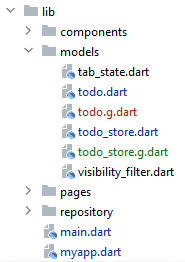
\includegraphics[width=0.4\textwidth]{Images/struttura_cartelle_mobx.png}
    \caption{Shows the final folders structure for the MobX implementation of the Todos app}
    \label{fig:struttura_cartelle_mobx}
\end{figure}
Figure \ref{fig:widget_tree_structure_mobx} represents the widget's tree structure for the MobX final application. 
\begin{figure}[H]
    \centering
    \subfloat[Widgets tree structure \textit{todos }tab \label{fig:todos_tab_UI}]{
        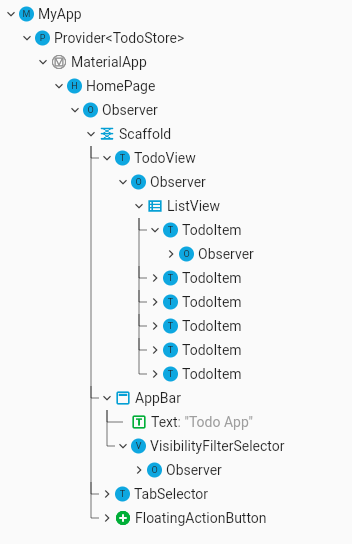
\includegraphics[scale=0.6]{Images/albero_mobx_todos.png}
    }
    \quad
    \subfloat[Widgets tree structure \textit{stats }tab\label{fig:todos_tab_tree}]{
        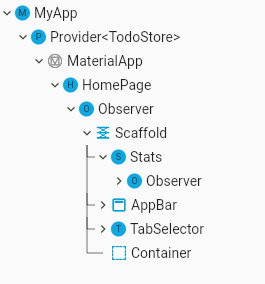
\includegraphics[scale=0.6]{Images/albero_mobx_stats.png}
    }
    \caption{Shows the widgets tree structure for MobX Todos app}
    \label{fig:widget_tree_structure_mobx}
\end{figure}
